\documentclass{egpubl}
\usepackage{eg2027}

\ConferenceSubmission

\usepackage[T1]{fontenc}
\usepackage{dfadobe}
\usepackage{cite}
\BibtexOrBiblatex
\electronicVersion
\PrintedOrElectronic
\ifpdf
  \usepackage[pdftex]{graphicx}
  \pdfcompresslevel=9
\else
  \usepackage[dvips]{graphicx}
\fi
\usepackage{egweblnk}

\input{extra_pkgs}

\usepackage{amsmath}
\usepackage{amssymb}
\usepackage{multirow}
\usepackage{tabularx}
\usepackage{tikz}
\usetikzlibrary{arrows.meta,positioning,fit,shapes.geometric}

\newcommand{\method}{Relation-Grounded Floor Repair}
\newcommand{\fp}{Floor-Prior}
\newcommand{\eg}{e.g.,\ }
\newcommand{\ie}{i.e.,\ }

\title{Repairing Graph-to-Layout Relation Grounding in Instruction-Guided 3D Indoor Scene Generation}

\author[SUBMISSION ID]{SUBMISSION ID}

\begin{document}

\maketitle

\begin{abstract}
Instruction-guided 3D indoor scene generation requires final layouts to realize the spatial relations requested by a user, not merely to generate plausible object sets or symbolic scene graphs. We show that a pretrained InstructScene pipeline exhibits a graph-to-layout grounding gap: explicit relations in the instruction can be lost when a generated scene graph is decoded into continuous object placements. We introduce \method, a training-free, safety-aware verifier-repair framework that parses explicit spatial relations, matches them to generated objects, verifies whether final layouts satisfy them, and applies bounded floor-plane repairs while preserving object height. On a frozen 531-scene evaluation spanning the existing InstructScene bedroom, living-room, and dining-room validation splits, collision-gated \fp{} obtains 0.6399 realized relation accuracy, compared with 0.6254 for the mean of three exact movement-matched random controls (gain 1.44 percentage points; paired scene-level bootstrap 95\% confidence interval, 0.75 to 2.20 points). The selected layouts contain 1,061 FCL mesh-collision pairs, compared with 1,075 for the original layouts. The gain over the original InstructScene baseline is smaller and its confidence interval includes zero; our evidence therefore supports a bounded claim of relation-aware control beyond matched random movement, not superiority to every comparator.
\ccsdesc[500]{Computing methodologies~Computer graphics}
\ccsdesc[300]{Computing methodologies~Spatial and physical reasoning}
\ccsdesc[300]{Computing methodologies~Scene understanding}
\printccsdesc
\begin{keywords}
3D indoor scene generation, spatial relations, layout repair, geometric verification
\end{keywords}
\end{abstract}

\section{Introduction}

Text-conditioned 3D indoor scene generation is useful for embodied AI, simulation, game production, and interactive design. In these settings, spatial language is not decorative. If a prompt asks for a nightstand behind a bed or a coffee table to the right of a side table, the generated layout must realize that relation in geometry. Recent indoor scene generators synthesize plausible object arrangements from scene categories, floor plans, scene graphs, or text~\cite{paschalidou2021atiss,wang2021sceneformer,tang2024diffuscene,lin2024instructscene}. However, a symbolic relation that appears in an intermediate graph does not guarantee that the final continuous layout satisfies the requested relation.

This paper studies this failure mode in InstructScene~\cite{lin2024instructscene}, an instruction-driven 3D indoor scene synthesis pipeline with a semantic graph prior. We identify a \emph{graph-to-layout grounding gap}: an instruction may contain explicit spatial relations, and the generator may produce plausible scenes, yet the decoded object centers can violate the requested relations. Rather than train a new generator or introduce a new benchmark, we ask whether a lightweight verifier-repair layer can improve relation realization using the existing InstructScene checkpoints, validation prompts, and evaluation protocol.

We propose \method, a plug-in final-layout relation grounding module. Given a generated layout and its source instruction, the module extracts explicit spatial relation triples, matches the triples to generated object categories, verifies whether the floor-plane geometry satisfies them, and repairs object translations when a relation is violated. The final design repairs only the horizontal floor plane, preserving the vertical coordinate of every object. This detail matters in practice: early 3D repair variants can improve relation metrics while producing visually implausible scenes with floating furniture. Our \fp{} variant selects among bounded candidate repairs using relation satisfaction and overlap-aware scoring, and a collision-gated verifier can fall back to the baseline layout whenever mesh collision increases.

Our experiments use the original InstructScene bedroom, living-room, and dining-room validation splits. A frozen run generated one layout for each of 531 validation scenes and evaluated 808 explicit target relations with an independent evaluator. Collision-gated \fp{} attains 0.6399 relation accuracy, compared with 0.6349 for the original layouts, 0.6254 for the mean of three exact movement-matched random controls, and 0.6411 for a budget-matched generic relation optimizer. Paired scene-level bootstrap intervals support the comparison with matched random movement but include zero for the comparisons with the original baseline and the generic optimizer. The collision gate selects 492 repaired layouts and falls back to 39 original layouts; the selected set contains 1,061 mesh-collision pairs versus 1,075 for the original set.

Our contribution is not a claim of first relation-aware 3D scene generation, nor a claim that a post-generation layer replaces stronger full generators. Strong related systems use scene graphs, semantic dependency graphs, language models, and optimization to reason about spatial constraints~\cite{feng2023layoutgpt,yang2024holodeck,zhai2023commonscenes,bucher2026respace,gao2026sdgscenes}. Instead, this paper makes a narrower and reproducible claim:
\begin{itemize}[leftmargin=1.5em]
    \item We identify and quantify a graph-to-layout grounding gap in an existing instruction-guided 3D scene generator.
    \item We introduce a training-free relation-grounded post-generation control framework: relation parsing, object matching, geometric verification, bounded floor-plane repair, and collision-gated validation.
    \item We operationalize bounded post-generation control through height preservation, movement limits, and a per-scene mesh-collision non-worsening gate.
\end{itemize}

\begin{figure}[t]
\centering
\resizebox{0.98\linewidth}{!}{
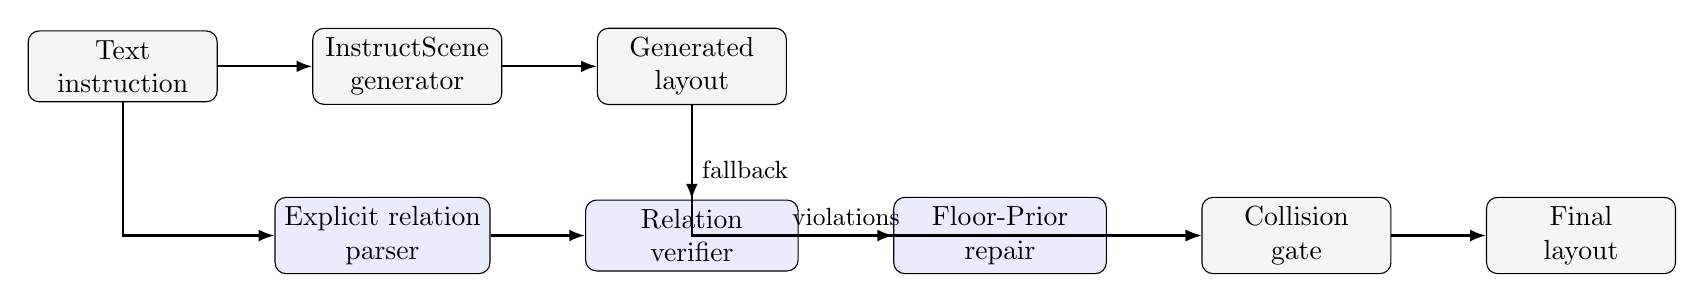
\begin{tikzpicture}[
  node distance=1.2cm,
  block/.style={draw, rounded corners, align=center, minimum width=2.4cm, minimum height=0.9cm, fill=gray!8},
  ours/.style={draw, rounded corners, align=center, minimum width=2.7cm, minimum height=0.9cm, fill=blue!8},
  arrow/.style={-{Latex[length=2mm]}, thick}
]
\node[block] (prompt) {Text\\instruction};
\node[block, right=of prompt] (gen) {InstructScene\\generator};
\node[block, right=of gen] (layout) {Generated\\layout};
\node[ours, below=of layout] (verify) {Relation\\verifier};
\node[ours, left=of verify] (parse) {Explicit relation\\parser};
\node[ours, right=of verify] (repair) {\fp{}\\repair};
\node[block, right=of repair] (gate) {Collision\\gate};
\node[block, right=of gate] (out) {Final\\layout};
\draw[arrow] (prompt) -- (gen);
\draw[arrow] (gen) -- (layout);
\draw[arrow] (prompt) |- (parse);
\draw[arrow] (layout) -- (verify);
\draw[arrow] (parse) -- (verify);
\draw[arrow] (verify) -- node[above, font=\small]{violations} (repair);
\draw[arrow] (repair) -- (gate);
\draw[arrow] (layout) |- node[pos=0.25, right, font=\small]{fallback} (gate);
\draw[arrow] (gate) -- (out);
\end{tikzpicture}}
\caption{\textbf{\method{} overview.} We keep the pretrained InstructScene generator fixed, parse explicit spatial relations from the input instruction, match them to generated objects, verify the final continuous layout, and repair violated relations in the floor plane while preserving object height. The collision gate falls back to the original layout when mesh collision would increase.}
\label{fig:overview}
\end{figure}

\section{Related Work}

\paragraph*{Indoor scene synthesis.}
3D-FRONT~\cite{fu20213dfront} and 3D-FUTURE~\cite{fu20203dfuture} provide large-scale room layouts and textured furniture assets that underpin much recent indoor scene synthesis work. ATISS~\cite{paschalidou2021atiss} models indoor scenes as unordered sets generated autoregressively. SceneFormer~\cite{wang2021sceneformer} uses transformers to generate indoor scenes conditioned on room layouts. DiffuScene~\cite{tang2024diffuscene} uses denoising diffusion over unordered object attributes. These methods focus on plausible and diverse indoor layouts; our work focuses on whether explicit natural-language relations are realized in the final layout of an instruction-conditioned pipeline.

\paragraph*{Text and graph conditioned scene generation.}
InstructScene~\cite{lin2024instructscene} is our direct baseline because it synthesizes 3D indoor scenes from natural language instructions with a semantic graph prior. CommonScenes~\cite{zhai2023commonscenes} converts scene graphs into commonsense 3D scenes with scene graph diffusion. LayoutGPT~\cite{feng2023layoutgpt} uses large language models as visual planners for layouts, including spatial and numerical constraints. Holodeck~\cite{yang2024holodeck} uses language models and 3D assets to generate embodied AI environments, including spatial constraints for object placement. These works show that language and structured relations are useful interfaces for scene generation. Our contribution is complementary: we evaluate and repair the final realized relation after a pretrained instruction-to-scene pipeline has produced a layout.

\paragraph*{Strong relation-aware systems.}
ReSpace~\cite{bucher2026respace} is a close text-driven indoor scene synthesis and editing framework based on structured scene representations and a specialized language model. SDGScenes~\cite{gao2026sdgscenes} uses a semantic dependency graph, VLM-derived commonsense constraints, and nonlinear constrained optimization to align scenes with user intent. These systems overlap with the broad goal of relation- and intent-aware 3D generation. We therefore do not claim to outperform them or to be the first relation-aware method. Our current fair comparison is the original InstructScene output under the same validation prompts and checkpoints; ReSpace and SDGScenes require a shared protocol before direct numerical claims are appropriate. Put differently, we do not replace strong generators; we study a plug-in final-layout relation grounding layer for an existing instruction-guided generator.

\paragraph*{Relation-grounded evaluation.}
RelScene~\cite{ye2024relscene} introduces a benchmark and baseline for evaluating spatial relations in text-driven 3D scene generation. It reinforces the need to measure whether text-specified relations are present in generated scenes, but its dataset, relation definitions, training setting, and metrics differ from the frozen InstructScene protocol used here. We therefore use RelScene as evaluation context rather than placing its reported numbers in our direct-comparison table.

\section{Method}

\subsection{Problem Setup}

Let an instruction-conditioned generator produce a scene layout
\[
  S = \{(c_i, t_i, s_i, r_i, m_i)\}_{i=1}^{N},
\]
where object $i$ has category $c_i$, translation $t_i \in \mathbb{R}^{3}$, size $s_i$, yaw rotation $r_i$, and optionally a retrieved mesh identifier $m_i$. The instruction text $x$ contains a set of explicit spatial relations
\[
  R(x) = \{(c_a, p, c_b)\},
\]
where predicate $p$ may be left-of, right-of, in-front-of, behind, near, far, above, or below. The repairable set contains the six horizontal direction and distance predicates. Above and below remain part of evaluation, but the repair never changes them because every vertical coordinate is preserved. The goal is to produce a repaired layout $S'$ that improves the realized satisfaction of $R(x)$ while limiting movement and mesh-collision side effects.

\subsection{Explicit Relation Extraction and Matching}

We use a deliberately simple rule-based parser to extract explicit spatial phrases. This choice makes the method transparent and keeps the benchmark unchanged. The parser output is noisy but sufficient to drive the formal parsed-relation verifier evaluated below. The parser is not intended to solve implicit commonsense reasoning; prompts that require latent affordance or support reasoning are outside the current claim.

For each parsed triple, the verifier finds generated objects whose class labels match the subject and object categories after deterministic alias normalization. When multiple instances match, the nearest pair in the floor plane is selected, with object indices breaking distance ties. For experimental comparison, the independent evaluator performs this selection once on the original layout and freezes the same instance indices across all variants. This prevents a repaired method from receiving credit by switching to an easier pair. If either target category is absent, the relation is marked missing and remains in the denominator.

\subsection{Relation Verification}

For a candidate object pair $(i,j)$, define $\Delta x=t_i^x-t_j^x$, $\Delta y=t_i^y-t_j^y$, $\Delta z=t_i^z-t_j^z$, and $d_{xz}=\sqrt{\Delta x^2+\Delta z^2}$. With directional margin $\epsilon=0.05$\,m, close threshold $d_c=0.75$\,m, and far threshold $d_f=1.60$\,m, the independent evaluator uses
\[
\begin{aligned}
\text{left}(i,j)&\Leftrightarrow \Delta x<-\epsilon,&
\text{right}(i,j)&\Leftrightarrow \Delta x>\epsilon,\\
\text{front}(i,j)&\Leftrightarrow \Delta z>\epsilon,&
\text{behind}(i,j)&\Leftrightarrow \Delta z<-\epsilon,\\
\text{near}(i,j)&\Leftrightarrow d_{xz}\le d_c,&
\text{far}(i,j)&\Leftrightarrow d_{xz}\ge d_f.
\end{aligned}
\]
Above and below analogously test $\Delta y>\epsilon$ and $\Delta y<-\epsilon$. We report exact selected-relation accuracy, counting a target correct only when its frozen object pair satisfies the corresponding test.

\subsection{Direct Height-Preserving Repair}

The direct repair baseline moves an object in the floor plane to satisfy a violated relation. It preserves the original height coordinate:
\[
  t_i' = (t_i^x + \delta_x, \; t_i^y, \; t_i^z + \delta_z).
\]
This repair can satisfy a target relation by moving an object substantially and can increase mesh collision. We therefore use direct height-preserving repair only as a development diagnostic, not as the paper-facing method or as evidence for the formal result.

\subsection{Floor-Prior Repair}

The \fp{} repair constrains relation repair with scene priors. For a violated relation, the method proposes candidate translations with interpolation strengths $\alpha \in \{0.25,0.5,0.75,1.0\}$, clamps movement by a maximum radius, and scores candidates by relation satisfaction and coarse overlap penalties. The chosen candidate must improve the relation while keeping the motion bounded. In all variants, the vertical coordinate remains unchanged.

\begin{algorithm}[t]
\caption{\fp{} relation repair}
\label{alg:floor-prior}
\DontPrintSemicolon
\KwIn{Layout $S$, parsed relations $R(x)$, thresholds $d_{\mathrm{close}}, d_{\mathrm{far}}$, max movement $\rho$, passes $K$}
\KwOut{Repaired layout $S'$}
$S' \leftarrow S$\;
\For{$k=1$ \KwTo $K$}{
  \ForEach{$(c_a,p,c_b) \in R(x)$}{
    $(i,j) \leftarrow$ nearest matching object pair in the $x/z$ plane\;
    \If{$p$ is already satisfied by $(i,j)$}{continue}
    $\mathcal{C} \leftarrow$ bounded floor-plane candidate translations for object $i$\;
    Score each $c \in \mathcal{C}$ by relation satisfaction and overlap penalty\;
    Apply the best candidate, preserving $t_i^y$\;
  }
}
\Return{$S'$}\;
\end{algorithm}

\subsection{Collision-Gated Selection}

For mesh-aware evaluation, we load the retrieved 3D-FUTURE meshes and compute FCL mesh-collision pair counts using a trimesh collision manager. The collision-gated variant keeps the repaired scene only when the repaired mesh collision pair count does not exceed the baseline count; otherwise it falls back to the baseline layout for that scene. This gate is a verifier-selection layer and should be described explicitly.

\section{Experiments}

\subsection{Experimental Setup}

We evaluate one generated layout for every scene in the existing InstructScene validation splits: 162 bedrooms, 192 living rooms, and 177 dining rooms (531 scenes in total). We use the official pretrained SG diffusion VQ object-feature checkpoints at epochs 1999, 1459, and 1239, respectively, and a single frozen generator seed. The main configuration uses parsed relations, two bounded floor-plane repair passes, a maximum movement of 1.8\,m, close and far thresholds of 0.75 and 1.6\,m, and mesh-collision gating. An independent evaluator that does not import the repair or optimization modules scores all 808 target relations. Missing target objects (93 cases per variant) remain in the denominator, and no predicate is silently discarded.

We compare collision-gated \fp{} with the original InstructScene layout, three random controls that exactly match each object's horizontal movement magnitude, and a generic relation optimizer constrained by the same movement budget. Statistical comparisons use paired scene-level percentile bootstrap intervals. The frozen primary gate is the relation-weighted difference between our method and the mean of the three movement-matched random controls, using 10,000 paired resamples and seed 20260816. A 50,000-round room-stratified analysis serves as a sensitivity check rather than a second acceptance criterion.

\subsection{Evaluator Validation and Control Construction}

The independent evaluator does not import the repair, candidate-scoring, or fallback modules. On an adjudicated human subset, 79 relations were binary-evaluable after coordinate and missing-pair checks; evaluator agreement with the human labels was 0.823, with precision 0.897 and recall 0.867 for the satisfied class. This check does not establish perceptual scene quality, but it tests that the coordinate rules used for the formal tables correspond reasonably well to human judgments of the displayed object pairs.

For scene $s$ and object $i$, let $b_{si}=\lVert t^{\mathrm{main}}_{si}-t^{\mathrm{base}}_{si}\rVert_{xz}$ be the movement budget induced by the frozen main output. Each random control translates the object by exactly $b_{si}$ in a deterministic pseudo-random direction; three seeds test sensitivity to direction. The generic optimizer processes the frozen relations once and moves the relation subject toward the nearest satisfying boundary, clipping its displacement by $b_{si}$. It does not use \fp{} candidate scoring or the collision gate. Thus, the controls share the final layouts, target pairs, evaluator, and per-object movement budgets while varying whether movement direction is random, relation-directed, or \fp{}-selected.

\subsection{Protocol Comparability}

Table~\ref{tab:protocol} separates direct evidence from cross-protocol context. Entry into a direct numerical comparison requires the same validation scenes and prompts, object representation and taxonomy, target-pair policy, relation thresholds, missing-target policy, and evaluator. Only the original output, our repair, and the movement-budget controls meet these conditions. ReSpace and SDGScenes are broader generation systems under their own protocols; RelScene is a dedicated relation benchmark. They are therefore strong references, not ranked baselines in our main table.

\begin{table*}[t]
\centering
\scriptsize
\caption{Protocol comparability. ``Aligned'' requires the same InstructScene validation split, layout representation, target relations, thresholds, missing-target policy, and independent evaluator. Cross-protocol methods are included to state the reproducibility boundary, not to imply a numerical ranking.}
\label{tab:protocol}
\begin{tabularx}{\textwidth}{p{2.05cm}X p{2.25cm}p{2.9cm}p{1.1cm}p{2.15cm}X}
\toprule
Method & Native input/data & Output & Relation and physical constraints & Aligned? & Local status & Role in this paper \\
\midrule
Official InstructScene~\cite{lin2024instructscene} & Natural-language instruction; InstructScene validation split & Category, translation, size, yaw & Learned semantic graph prior and layout decoder & Yes & Runnable; frozen outputs & Direct baseline \\
Collision-gated \fp{} & Original output plus parsed explicit relations & Same layout with bounded $x/z$ edits & Fixed verifier, floor prior, movement bound, FCL non-worsening gate & Yes & Runnable; frozen outputs & Main method \\
Random/generic controls & Original output plus frozen target pairs & Same layout under per-object movement budgets & Random direction or one-pass relation projection; no \fp{} scoring & Yes & Runnable; three random seeds & Direct controls \\
ReSpace~\cite{bucher2026respace} & Text-driven synthesis/editing; native structured-scene protocol & Autoregressive scene representation and assets & Learned addition/editing with geometry-aware evaluation & No & Native-protocol engineering only & Strong related system; no ranking \\
SDGScenes~\cite{gao2026sdgscenes} & Implicit user intent and semantic dependency graph; native protocol & Category, size, position, yaw & SDG-guided VLM plus collision, boundary, reachability, and commonsense constraints & No & Official runnable release not verified & Strong related system; no ranking \\
RelScene~\cite{ye2024relscene} & Text-driven relation benchmark built from its own annotations & Benchmark-specific scene representation & Explicit relation labels and relation-consistency metrics & No & Evaluation reference & Metric context; not a generator baseline \\
\bottomrule
\end{tabularx}
\end{table*}

We also retain a separately archived, non-official SDGScenes-inspired constrained-optimization smoke run. It covers the same 531 room instances but uses an earlier 708-target relation export and a simpler satisfaction metric, rather than the frozen 808-target independent-evaluator protocol. Its numbers are therefore excluded from Tables~\ref{tab:main} and~\ref{tab:controls}; the frozen generic optimizer is the appropriate same-protocol optimization control.

\subsection{Main Results}

Table~\ref{tab:main} reports the independently evaluated formal run. Collision-gated \fp{} has a positive point difference from the original layout in each room and an overall gain of 0.50 percentage points. The paired overall confidence interval for this comparison includes zero, so these point differences are descriptive rather than evidence of statistical superiority to the original InstructScene baseline.

Figure~\ref{fig:formal-qualitative} provides deterministic qualitative evidence from the same frozen formal artifacts. To avoid cherry-picking, examples are selected by a fixed rule: the lexicographically first evaluated baseline-fail/gated-pass relation with nonzero horizontal movement in each room type, followed by the first repaired relation that still fails. The first three examples show realized relation changes, while the final example makes the remaining failure mode explicit.

\begin{figure*}[t]
\centering
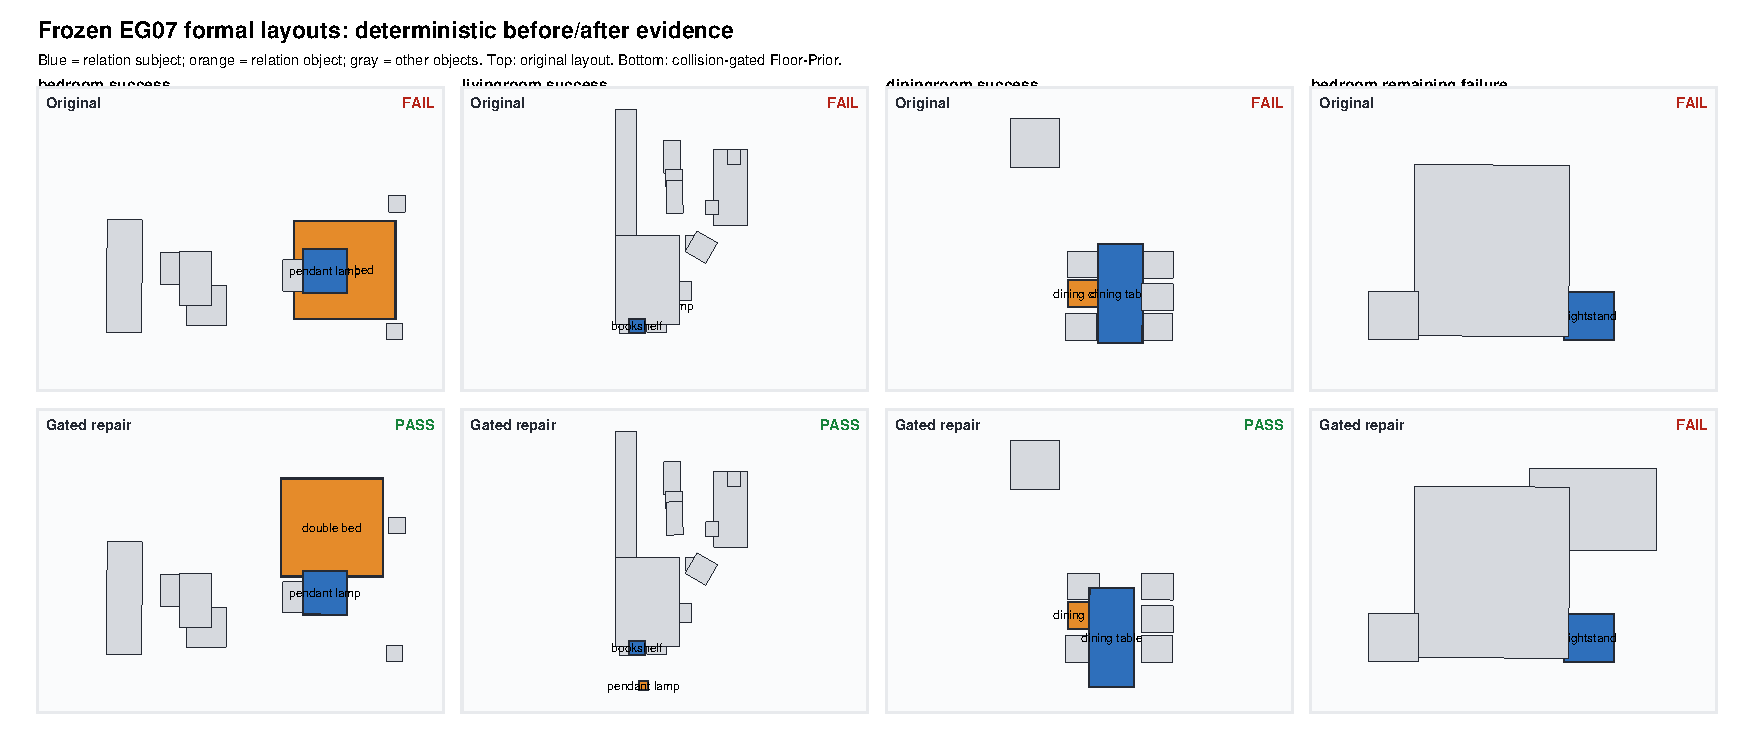
\includegraphics[width=\textwidth]{figures/eg11_formal_qualitative.pdf}
\caption{\textbf{Deterministically selected formal before/after evidence.} Blue and orange denote the evaluated relation subject and object; gray rectangles denote other objects. The top row shows the original InstructScene layouts and the bottom row shows collision-gated \fp{}. The three room-specific examples change from relation failure to success; the rightmost example remains a failure after repair. These are floor-plane layout projections from the frozen EG07 artifact, not photorealistic renderings or evidence of universal visual improvement.}
\label{fig:formal-qualitative}
\end{figure*}

\begin{table}[t]
\centering
\caption{Formal 531-scene relation results from the independent evaluator. Missing targets remain in the denominator. Gains are percentage-point differences from the original InstructScene layouts and are descriptive at room level.}
\label{tab:main}
\setlength{\tabcolsep}{4pt}
\begin{tabular}{lrrrr}
\toprule
Room & Scenes & Relations & Baseline & Gated \fp{} \\
\midrule
Bedroom & 162 & 245 & 0.7265 & 0.7306 \\
Living room & 192 & 294 & 0.6054 & 0.6122 \\
Dining room & 177 & 269 & 0.5836 & 0.5874 \\
\textbf{Overall} & \textbf{531} & \textbf{808} & \textbf{0.6349} & \textbf{0.6399} \\
\bottomrule
\end{tabular}
\end{table}

\subsection{Movement-Matched Controls and Uncertainty}

Table~\ref{tab:controls} tests whether relation changes can be explained by movement alone. Collision-gated \fp{} exceeds every movement-matched random seed and their mean. Against the random-seed mean, the gain is 1.44 percentage points and the frozen paired bootstrap interval is [0.75, 2.20] points. Both the scene-unweighted and relation-weighted intervals are positive for all three random seeds and their mean. By contrast, the intervals for the original baseline and the budget-matched generic optimizer include zero. The generic optimizer's point estimate is 0.6411, slightly above our 0.6399; we therefore make no superiority claim for that comparison.

\begin{table}[t]
\centering
\caption{Overall fair-comparison results. Gain and 95\% confidence interval (CI) are for collision-gated \fp{} minus the listed control, in percentage points, under the frozen paired scene-level relation-weighted bootstrap protocol.}
\label{tab:controls}
\setlength{\tabcolsep}{4pt}
\begin{tabular}{lrrr}
\toprule
Control & Accuracy & Gain & 95\% CI \\
\midrule
Original baseline & 0.6349 & +0.50 & [$-0.13$, 1.22] \\
Random movement, seed 0 & 0.6225 & +1.73 & [0.75, 2.83] \\
Random movement, seed 1 & 0.6250 & +1.49 & [0.61, 2.50] \\
Random movement, seed 2 & 0.6287 & +1.11 & [0.37, 1.96] \\
\textbf{Random-seed mean} & \textbf{0.6254} & \textbf{+1.44} & \textbf{[0.75, 2.20]} \\
Generic optimizer & 0.6411 & $-0.12$ & [$-0.63$, 0.38] \\
\bottomrule
\end{tabular}
\end{table}

\subsection{Collision-Gate Accounting and Safety}

The gate accepted 492 repaired layouts and selected the original layout for the remaining 39 scenes. Every one of the 531 scenes had mesh evidence, and no scene bypassed the gate. Across the selected set, the FCL collision-pair total was 1,061, compared with 1,075 for the original layouts. This aggregate non-worsening result supports the safety claim; it does not imply that collision-free generation has been solved.

\begin{table}[t]
\centering
\caption{Collision-gate accounting in the formal run. Each scene has exactly one terminal gate decision.}
\label{tab:gated}
\begin{tabular}{lrrr}
\toprule
Room & Repair selected & Baseline fallback & Total \\
\midrule
Bedroom & 154 & 8 & 162 \\
Living room & 174 & 18 & 192 \\
Dining room & 164 & 13 & 177 \\
\textbf{Overall} & \textbf{492} & \textbf{39} & \textbf{531} \\
\bottomrule
\end{tabular}
\end{table}

Room-level sensitivity intervals for the primary random-mean comparison are positive for bedrooms and dining rooms. The living-room lower bound is exactly zero, so we do not claim a strictly positive effect in every room. The aggregate primary interval remains positive under both the frozen 10,000-round protocol and an additional 50,000-round room-stratified sensitivity analysis.

\section{Discussion}

The results support a narrow conclusion: relation-aware post-generation control performs better than moving objects by matched random directions under the same movement magnitudes. This comparison isolates structure in the repair direction from movement alone. The smaller and statistically inconclusive difference from the original InstructScene layouts shows that the formal effect should not be described as a broad performance breakthrough. Likewise, the generic optimizer's similar point estimate indicates that the present evidence does not isolate a unique advantage over generic budgeted constraint optimization.

The results also reveal an evaluation lesson. Reporting only symbolic scene graph correctness can miss failures in the final continuous layout. Conversely, reporting only visual examples can hide whether the requested relation is actually satisfied. A relation-aware scene generation benchmark should evaluate instruction parsing, graph-level relation accuracy, final layout relation accuracy, and geometric side effects separately.

The protocol analysis also clarifies the intended plug-in scope. A generator can use the verifier-repair layer only if it exposes object categories and continuous layout attributes and if its language relations can be mapped to the evaluator predicates. This makes transfer to another generator technically plausible, but Table~\ref{tab:protocol} is not evidence that such transfer already succeeds.

\section{Limitations}

The current method targets explicit spatial relations. It does not handle all implicit commonsense requirements, such as affordance, reachability, support, or task-specific functional arrangements. The parser is rule-based and intentionally simple; stronger language parsing may further improve recall and precision. The collision-gated variant is a post-hoc verifier-selection layer, not an end-to-end collision-aware generator, and a lower aggregate collision-pair count does not imply collision-free scenes. The formal run uses one generated layout per validation scene at a single generator seed. Moreover, the comparisons with the original baseline and the generic optimizer are statistically inconclusive, and the living-room sensitivity interval against the random-seed mean touches zero. Finally, we do not claim superiority over ReSpace, SDGScenes, or other strong related methods without a shared evaluation protocol. The lightweight public evidence package contains the complete per-scene relation tables used for statistics but not the three original room-level generator JSON files; this is a remaining provenance gap for full generator-to-statistics reconstruction.

\section{Conclusion}

We presented \method, a training-free verifier-repair layer for instruction-guided 3D indoor scene generation. The method addresses a graph-to-layout grounding gap in InstructScene by parsing explicit spatial relations, verifying final layout geometry, and applying bounded floor-plane repairs that preserve object heights. On the frozen 531-scene evaluation, collision-gated \fp{} improved relation accuracy over exact movement-matched random controls by 1.44 percentage points (95\% confidence interval, 0.75 to 2.20 points) while keeping the selected layouts' FCL collision-pair total no higher than the original layouts. The evidence supports structured post-generation control beyond random movement, while leaving superiority over the original generator and a generic optimizer unresolved.

\section*{Reproducibility Notes}

An anonymized evidence package contains the formal 531-scene layouts, validation records, independent relation evaluation, movement-matched controls, final metrics, paired statistics, and file checksums. Third-party datasets, checkpoints, environments, and the three original room-level generator JSON files are not included in the lightweight package. The separate SDGScenes-inspired smoke archive is retained for feasibility auditing but is deliberately excluded from the formal 808-relation result tables.

\bibliographystyle{eg-alpha-doi}
\bibliography{references}

\end{document}
